\documentclass[aspectratio=169, 11pt]{beamer}

% --- Packages & Setup ---
\usepackage[utf8]{inputenc}
\usepackage[T1]{fontenc}
\usepackage{xcolor}
\usepackage{booktabs}
\usepackage{graphicx}
\usepackage{tikz}
\usepackage{amsmath,amssymb}
\usetikzlibrary{calc, arrows.meta, positioning, shapes.geometric, fit}

\graphicspath{{../}{./}}

% Try loading Open Sans; fallback if missing
\IfFileExists{opensans.sty}{\usepackage[default,scale=0.95]{opensans}}{}

% --- Branding Colors ---
\definecolor{amritaMaroon}{HTML}{A4123F}
\definecolor{macroBlue}{HTML}{2B5B84}
\definecolor{microOrange}{HTML}{D97925}
\definecolor{darkGreen}{HTML}{2E7D32}
\definecolor{lightGray}{HTML}{F5F5F5}
\definecolor{medGray}{HTML}{CCCCCC}

% --- Theme Setup ---
\usetheme{Madrid}
\usecolortheme[named=amritaMaroon]{structure}
\setbeamertemplate{navigation symbols}{}
\setbeamertemplate{footline}[frame number]

\begin{document}

% =====================================================================
%  TITLE SLIDE
% =====================================================================
\begin{frame}
    \begin{tikzpicture}[remember picture,overlay]
        \node[fill=amritaMaroon, text=white, font=\bfseries\footnotesize, anchor=north east, rounded corners=2pt, inner sep=5pt]
        at ($(current page.north east) + (-0.2cm,-0.2cm)$)
        {Type 1: Research Project};
    \end{tikzpicture}

    \centering
    \includegraphics[width=2.8cm]{logo.png}
    \vspace{0.1cm}

    {\large \textbf{\textcolor{amritaMaroon}{Trajectory-Driven Cooperative Coevolutionary Algorithms}}} \\
    {\large \textbf{\textcolor{amritaMaroon}{for Strategy Optimization in Dynamic RTS Environments}}} \\
    \vspace{0.05cm}
    {\footnotesize \textbf{23CSE498 -- Project Phase 2 (Panel Review 1)} \quad | \quad \textbf{Team Number: [XX]}} \\
    \vspace{0.15cm}

    \begin{table}
        \centering
        \footnotesize
        \renewcommand{\arraystretch}{1.05}
        \begin{tabular}{|c|c|l|}
            \hline
            \textbf{S.No} & \textbf{Register Number} & \textbf{Student Name} \\
            \hline
            1 & CB.EN.U4CSE23XXX & Student Name 1 \\
            \hline
            2 & CB.EN.U4CSE23XXX & Student Name 2 \\
            \hline
            3 & CB.EN.U4CSE23XXX & Student Name 3 \\
            \hline
            4 & CB.EN.U4CSE23XXX & Student Name 4 \\
            \hline
        \end{tabular}
    \end{table}
    \vspace{0.1cm}

    {\footnotesize Guide: \textbf{Guide Name}, Designation, Department of CSE} \\
    \vspace{0.1cm}
    {\scriptsize \today}
\end{frame}

% =====================================================================
%  SLIDE 1: PROBLEM STATEMENT & ABSTRACT
% =====================================================================
\section{Problem Statement}
\begin{frame}{1. Problem Statement \& Abstract}
    \framesubtitle{Evolving Intelligent Agents for Real-Time Strategy Games}

    \textbf{\textcolor{amritaMaroon}{Problem Statement:}} \\[0.15cm]
    Developing AI agents for Real-Time Strategy (RTS) games that can \textbf{continuously adapt} to dynamic environments and evolving opponents remains an open challenge. Conventional approaches---including handcrafted heuristics, static GAs, and fixed-strategy selection---suffer from \textbf{catastrophic forgetting}, \textbf{premature convergence}, and inability to generalize across varying map topographies, opponent behaviors, and resource constraints.

    \vspace{0.3cm}
    \textbf{\textcolor{amritaMaroon}{Abstract:}} \\[0.15cm]
    We propose a family of \textbf{Trajectory-Driven Cooperative Coevolutionary Algorithms (TD-CCEA)} that evolve 20-dimensional continuous strategy vectors for the microRTS game engine. Unlike traditional GAs that rely on momentary fitness, our algorithms evaluate agents using \textbf{weighted performance histories} across multiple generations, enabling context-aware self-adapting mutation rates. We introduce two key variants---\textbf{SA-TDCCEA} (Sensitivity-Adaptive) and \textbf{CCE-TDCCEA} (Cooperative Co-Evolutionary)---and evaluate them on \textbf{dynamic 48$\times$48 maps with progressive BFS-validated blockades}, demonstrating superior adaptability, diversity preservation, and strategy optimization over baseline algorithms.
\end{frame}

% =====================================================================
%  SLIDE 2: RESEARCH GAPS (Phase 1 & Phase 2)
% =====================================================================
\section{Research Gaps}
\begin{frame}{2. Research Gaps Addressed (Phase 1 \& Phase 2)}
    \framesubtitle{From Discrete Strategy Selection to Continuous Co-Evolutionary Optimization}

    \begin{columns}[T]
        \column{0.48\textwidth}
        \textbf{\textcolor{amritaMaroon}{Phase 1 Research Gaps:}}
        \begin{itemize}\small
            \item Traditional GAs use \textbf{momentary (single-generation) fitness} $\rightarrow$ catastrophic forgetting.
            \item \textbf{Static mutation rates} across all dimensions $\rightarrow$ poor exploration--exploitation balance.
            \item Strategy space limited to \textbf{14 predefined scripts} (discrete) $\rightarrow$ no novel strategy creation.
            \item Agents evolved against \textbf{fixed opponents only} $\rightarrow$ no arms race or co-adaptation.
        \end{itemize}

        \column{0.48\textwidth}
        \textbf{\textcolor{amritaMaroon}{Phase 2 Contributions:}}
        \begin{itemize}\small
            \item \textbf{Trajectory Memory:} Fitness evaluated across \textit{all similar past environments}, not just the current generation.
            \item \textbf{Sensitivity-Adaptive Mutation (SA-TDCCEA):} Per-weight mutation rates based on measured influence.
            \item \textbf{Cooperative Co-Evolution (CCE-TDCCEA):} Macro (economy, 8D) and Micro (combat, 12D) evolved \textit{independently} and combined cooperatively.
            \item \textbf{Dynamic Environments:} Progressive blockades with BFS-validated path connectivity.
            \item \textbf{Competitive Co-Evolution:} Algorithms evolve \textit{against each other}, creating arms races.
        \end{itemize}
    \end{columns}
\end{frame}

% =====================================================================
%  SLIDE 3: METHODOLOGY & SOLUTION DESIGN
% =====================================================================
\section{Methodology \& Solution Design}
\begin{frame}{3. Methodology \& Solution Design}
    \framesubtitle{Rubric: Workflow, Architecture, Algorithms \& Evaluation Metrics (5 Marks)}

    \begin{columns}[T]
        \column{0.52\textwidth}
        \textbf{\textcolor{amritaMaroon}{Methodological Framework:}}
        \begin{itemize}\small
            \item \textbf{Game Engine:} microRTS (Java-based RTS simulator) with Python$\leftrightarrow$Java subprocess communication.
            \item \textbf{Strategy Representation:} 20-dimensional continuous weight vector $\boldsymbol{\theta} \in [0,1]^{20}$ controlling economy, unit production, and combat.
            \item \textbf{Core Algorithm:} TD-CCEA with centroid-based environment meta-state, trajectory memory $H_i$, and self-adaptive mutation.
            \item \textbf{Variants:} SA-TDCCEA (per-weight mutation), CCE-TDCCEA (macro/micro decomposition).
            \item \textbf{Evaluation Metrics:} Win rate (\%), convergence speed, diversity index, head-to-head Elo, Wilcoxon signed-rank test ($p < 0.05$).
        \end{itemize}

        \column{0.45\textwidth}
        \centering
        \small
        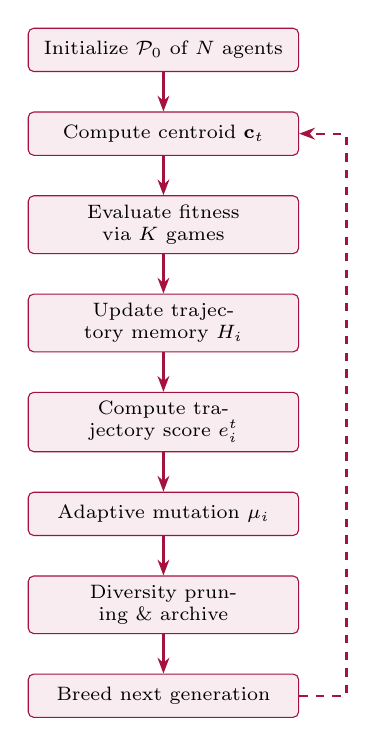
\begin{tikzpicture}[node distance=0.5cm, auto,
            block/.style={rectangle, draw=amritaMaroon, fill=amritaMaroon!8, text width=3.2cm, minimum height=0.55cm, align=center, font=\scriptsize, rounded corners=2pt},
            arrow/.style={-{Stealth[length=2mm]}, thick, amritaMaroon}]
            \node[block] (init) {Initialize $\mathcal{P}_0$ of $N$ agents};
            \node[block, below=of init] (cent) {Compute centroid $\mathbf{c}_t$};
            \node[block, below=of cent] (eval) {Evaluate fitness via $K$ games};
            \node[block, below=of eval] (traj) {Update trajectory memory $H_i$};
            \node[block, below=of traj] (score) {Compute trajectory score $e_i^t$};
            \node[block, below=of score] (mut) {Adaptive mutation $\mu_i$};
            \node[block, below=of mut] (prune) {Diversity pruning \& archive};
            \node[block, below=of prune] (breed) {Breed next generation};
            \draw[arrow] (init) -- (cent);
            \draw[arrow] (cent) -- (eval);
            \draw[arrow] (eval) -- (traj);
            \draw[arrow] (traj) -- (score);
            \draw[arrow] (score) -- (mut);
            \draw[arrow] (mut) -- (prune);
            \draw[arrow] (prune) -- (breed);
            \draw[arrow, dashed] (breed.east) -- ++(0.6,0) |- (cent.east);
        \end{tikzpicture}
    \end{columns}
\end{frame}

% =====================================================================
%  SLIDE 4: IMPLEMENTATION PROGRESS
% =====================================================================
\section{Implementation Progress}
\begin{frame}{4. Implementation Progress ($\approx$60\%) \& Module Functionality}
    \framesubtitle{Rubric: Core Modules Implemented, Functional \& Integrated (8 Marks)}
    \begin{itemize}
        \item \textbf{Implementation Status Overview ($\approx$60\% Completed):}
    \end{itemize}
    \vspace{-0.2cm}
    \begin{table}
        \centering
        \footnotesize
        \renewcommand{\arraystretch}{1.1}
        \begin{tabular}{p{3.8cm} p{5.0cm} c}
            \toprule
            \textbf{Module / Component} & \textbf{Current Implementation State} & \textbf{Status} \\
            \midrule
            microRTS Java Engine & EvolvedBrainAI (20-weight parameterized agent) & \textcolor{darkGreen}{Functional} \\
            Python$\leftrightarrow$Java IPC & Subprocess-based batch game runner (stdin/stdout) & \textcolor{darkGreen}{Functional} \\
            TD-CCEA Core & Centroid, trajectory memory, adaptive mutation, archive & \textcolor{darkGreen}{Functional} \\
            SA-TDCCEA & Sensitivity analysis + per-weight mutation rates & \textcolor{darkGreen}{Functional} \\
            CCE-TDCCEA & Macro/Micro sub-population split with cooperative eval & \textcolor{darkGreen}{Functional} \\
            Dynamic Environment & Progressive blockades + BFS path validation (48$\times$48) & \textcolor{darkGreen}{Functional} \\
            Head-to-Head Tournament & EVOLVED vs EVOLVED competitive co-evolution & \textcolor{darkGreen}{Integrated} \\
            Statistical Analysis & Wilcoxon test, ablation study, JSON export & \textcolor{blue}{In Progress} \\
            \bottomrule
        \end{tabular}
    \end{table}
    \vspace{0.1cm}
    \begin{itemize}\small
        \item \textbf{Core Functionality:} All 4 algorithms (CCE-TDCCEA, TD-CCEA, SA-TDCCEA, Std CCEA) co-evolve competitively on dynamic maps; 10-run statistical benchmarks executed.
    \end{itemize}
\end{frame}

% =====================================================================
%  SLIDE 5: TECHNICAL KNOWLEDGE & DESIGN DECISIONS
% =====================================================================
\section{Technical Knowledge}
\begin{frame}{5. Technical Knowledge \& Design Decisions}
    \framesubtitle{Rubric: Understanding of Methodology, Implementation \& Design Choices (5 Marks)}
    \begin{itemize}\small
        \item \textbf{Algorithmic Justification:} The 20-dimensional continuous weight space creates an \textit{infinite} strategy space (vs.\ 14 discrete scripts), enabling evolutionary discovery of novel behaviors unreachable by handcrafted heuristics.

        \item \textbf{Mathematical Formulation:}
        \begin{itemize}\footnotesize
            \item \textbf{Environment meta-state:} $\mathbf{c}_t = \frac{1}{N}\sum_{i=1}^{N}\boldsymbol{\theta}_i^t$
            \item \textbf{Dynamic similarity:} $\alpha_k = 1 - \frac{d(\mathbf{c}_t,\,\mathbf{c}_k)}{d_{\max}}$, \quad $\hat{\alpha}_k = \frac{\alpha_k}{\sum_j \alpha_j}$
            \item \textbf{Trajectory score:} $e_i^t = \sum_k \hat{\alpha}_k \cdot f_i^{(k)}$
            \item \textbf{Adaptive mutation:} $\mu_i = \mu_{\text{base}} \cdot (1 - e_i^t) + \epsilon$
        \end{itemize}

        \item \textbf{Design Trade-offs:}
        \begin{itemize}\footnotesize
            \item \textit{Complexity vs.\ Speed:} CCE-TDCCEA doubles the population count (2$\times$20) but converges faster by searching two smaller sub-spaces (8D + 12D vs.\ 20D).
            \item \textit{Diversity Pruning:} Redundant agents ($S(i,j) > 0.85$) and weak agents ($\bar{e}_i < 0.20$) are removed to prevent premature convergence.
            \item \textit{Archive ($\mathcal{A}_{\max}=15$):} Stores top-$m$ agents across generations to prevent catastrophic forgetting.
        \end{itemize}
    \end{itemize}
\end{frame}

% =====================================================================
%  SLIDE 6: CORE ALGORITHM --- TD-CCEA
% =====================================================================
\section{Algorithms}
\begin{frame}{6. Core Algorithm: TD-CCEA}
    \framesubtitle{Trajectory-Driven Cooperative Coevolutionary Algorithm}

    \begin{columns}[T]
        \column{0.55\textwidth}
        {\small
        \textbf{\textcolor{amritaMaroon}{Algorithm: TD-CCEA}} \\[0.2cm]
        \textbf{Input:} Population size $N$, games per eval $K$, generations $T_{\max}$, archive size $A_{\max}$ \\[0.1cm]
        \begin{enumerate}\footnotesize
            \item Initialize $\mathcal{P}_0$ of $N$ agents, archive $\mathcal{A} \leftarrow \emptyset$
            \item \textbf{for} $t = 1, 2, \ldots, T_{\max}$ \textbf{do}
            \begin{enumerate}\scriptsize
                \item[(a)] Compute centroid $\mathbf{c}_t = \frac{1}{N}\sum_{i=1}^{N}\boldsymbol{\theta}_i^t$
                \item[(b)] Evaluate fitness $f_i^t$ for all $\mathcal{O}_i$ via $K$ simulated games
                \item[(c)] Update trajectory: $H_i \leftarrow H_i \cup \{(f_i^t, \mathbf{c}_t)\}$; trim if $|H_i| > W$
                \item[(d)] Compute similarity weights $\alpha_k = 1 - \frac{d(\mathbf{c}_t, \mathbf{c}_k)}{d_{\max}}$
                \item[(e)] Normalize: $\hat{\alpha}_k = \frac{\alpha_k}{\sum_j \alpha_j}$; \quad Score: $e_i^t = \sum_k \hat{\alpha}_k \cdot f_i^{(k)}$
                \item[(f)] Adaptive mutation: $\mu_i = \mu_{\text{base}} \cdot (1 - e_i^t) + \epsilon$
                \item[(g)] Remove weak ($\bar{e}_i < \delta_f$) and redundant ($S > \delta_s$) agents
                \item[(h)] Update archive $\mathcal{A}$; breed offspring with Gaussian mutation
            \end{enumerate}
            \item \textbf{return} best $\mathcal{O}^* \in \mathcal{A}$
        \end{enumerate}
        }

        \column{0.42\textwidth}
        \centering
        \textbf{\textcolor{amritaMaroon}{Key Innovations:}} \\[0.15cm]
        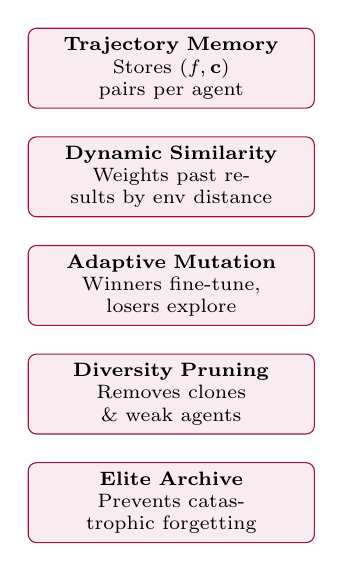
\begin{tikzpicture}[
            box/.style={rectangle, draw=amritaMaroon, fill=amritaMaroon!8, text width=3.4cm, minimum height=0.7cm, align=center, font=\scriptsize, rounded corners=3pt},
            node distance=0.35cm]
            \node[box] (tm) {\textbf{Trajectory Memory} \\ Stores $(f, \mathbf{c})$ pairs per agent};
            \node[box, below=of tm] (ds) {\textbf{Dynamic Similarity} \\ Weights past results by env distance};
            \node[box, below=of ds] (am) {\textbf{Adaptive Mutation} \\ Winners fine-tune, losers explore};
            \node[box, below=of am] (dp) {\textbf{Diversity Pruning} \\ Removes clones \& weak agents};
            \node[box, below=of dp] (ar) {\textbf{Elite Archive} \\ Prevents catastrophic forgetting};
        \end{tikzpicture}
    \end{columns}
\end{frame}

% =====================================================================
%  SLIDE 7: VARIANT 1 --- SA-TDCCEA
% =====================================================================
\begin{frame}{7. Variant: SA-TDCCEA (Sensitivity-Adaptive TD-CCEA)}
    \framesubtitle{Per-Weight Mutation Rates Based on Measured Influence}

    \begin{columns}[T]
        \column{0.48\textwidth}
        \textbf{\textcolor{amritaMaroon}{Phase 1: Sensitivity Analysis}}
        \begin{itemize}\small
            \item Set all 20 weights to baseline (0.5).
            \item For each weight $w_j$ independently:
            \begin{itemize}\footnotesize
                \item Set $w_j = 0.0$ (others at 0.5) $\rightarrow$ play games $\rightarrow$ win rate $r_{\text{low}}$
                \item Set $w_j = 1.0$ (others at 0.5) $\rightarrow$ play games $\rightarrow$ win rate $r_{\text{high}}$
            \end{itemize}
            \item \textbf{Influence:} $I_j = |r_{\text{high}} - r_{\text{low}}|$
        \end{itemize}

        \vspace{0.2cm}
        \textbf{\textcolor{amritaMaroon}{Phase 2: Adaptive Mutation}}
        \begin{itemize}\small
            \item High influence $\rightarrow$ \textbf{small} $\mu_j$ (fine-tune carefully)
            \item Low influence $\rightarrow$ \textbf{large} $\mu_j$ (explore freely)
            \item $\mu_j = 0.20 - \frac{I_j}{I_{\max}} \times 0.12 \quad \in [0.08, 0.20]$
        \end{itemize}

        \column{0.48\textwidth}
        \textbf{\textcolor{amritaMaroon}{Key Difference from Standard TD-CCEA:}}
        \begin{itemize}\small
            \item Standard: $\mu = 0.15$ \textbf{uniform} for all 20 weights.
            \item SA-TDCCEA: each weight $w_j$ gets its \textbf{own} $\mu_j$.
        \end{itemize}

        \vspace{0.2cm}
        \textbf{\textcolor{amritaMaroon}{Example Influence Ranking:}}
        {\footnotesize
        \begin{tabular}{lcc}
            \toprule
            \textbf{Weight} & \textbf{Influence} & $\boldsymbol{\mu_j}$ \\
            \midrule
            \texttt{aggression} & High & 0.08 \\
            \texttt{attack\_threshold} & High & 0.09 \\
            \texttt{light\_preference} & Med & 0.14 \\
            \texttt{second\_barracks} & Low & 0.19 \\
            \texttt{scout\_priority} & Low & 0.20 \\
            \bottomrule
        \end{tabular}
        }

        \vspace{0.15cm}
        {\scriptsize \textit{Analogy: Study harder for subjects that carry more marks.}}
    \end{columns}
\end{frame}

% =====================================================================
%  SLIDE 8: VARIANT 2 --- CCE-TDCCEA
% =====================================================================
\begin{frame}{8. Variant: CCE-TDCCEA (Cooperative Co-Evolutionary TD-CCEA)}
    \framesubtitle{Macro/Micro Decomposition with Independent Sub-Populations}

    \begin{columns}[T]
        \column{0.48\textwidth}
        \textbf{\textcolor{amritaMaroon}{Decomposition:}}
        \begin{itemize}\small
            \item \textbf{\textcolor{macroBlue}{Pop A --- Macro/Economy (8 weights):}} \\
            {\scriptsize \texttt{worker\_ratio}, \texttt{max\_workers}, \texttt{expand\_threshold}, \texttt{barracks\_timing}, \texttt{economy\_pressure}, \texttt{scout\_priority}, \texttt{second\_barracks}, \texttt{worker\_fight\_ratio}}
            \item \textbf{\textcolor{microOrange}{Pop B --- Micro/Combat (12 weights):}} \\
            {\scriptsize \texttt{light/heavy/ranged\_pref}, \texttt{aggression}, \texttt{attack\_threshold}, \texttt{defend\_radius}, \texttt{target\_priority}, \texttt{defense\_trigger}, \texttt{counter\_rush}, \texttt{tech\_switch}, \texttt{group\_attack}, \texttt{focus\_fire}}
        \end{itemize}

        \vspace{0.15cm}
        \textbf{\textcolor{amritaMaroon}{Cooperative Evaluation (``Handshake''):}}
        \begin{itemize}\footnotesize
            \item To evaluate a \textcolor{macroBlue}{Macro agent}: combine its 8 weights with the \textbf{best} \textcolor{microOrange}{Micro agent}'s 12 weights $\rightarrow$ play game $\rightarrow$ assign fitness to Macro.
            \item Vice versa for \textcolor{microOrange}{Micro agents}.
        \end{itemize}

        \column{0.48\textwidth}
        \textbf{\textcolor{amritaMaroon}{Why It Works:}}
        \begin{itemize}\small
            \item Searching two smaller spaces (8D + 12D) converges \textbf{exponentially faster} than one 20D space.
            \item A brilliant economy strategy is \textbf{not penalized} by a randomly bad combat behavior (and vice versa).
            \item Each sub-population has \textbf{its own} centroid, trajectory memory, archive, and pruning logic --- \textit{full TD-CCEA within each sub-population}.
        \end{itemize}

        \vspace{0.15cm}
        \centering
        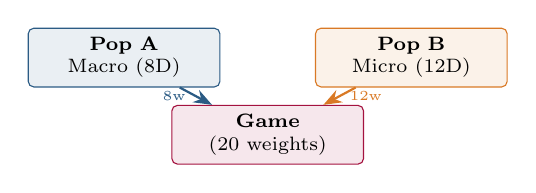
\begin{tikzpicture}[node distance=0.8cm,
            pop/.style={rectangle, draw, text width=2.2cm, minimum height=0.6cm, align=center, font=\scriptsize, rounded corners=2pt}]
            \node[pop, draw=macroBlue, fill=macroBlue!10] (a) {\textbf{Pop A} \\ Macro (8D)};
            \node[pop, draw=microOrange, fill=microOrange!10, right=1.2cm of a] (b) {\textbf{Pop B} \\ Micro (12D)};
            \node[pop, draw=amritaMaroon, fill=amritaMaroon!10, below=0.6cm of $(a)!0.5!(b)$] (game) {\textbf{Game} \\ (20 weights)};
            \draw[-{Stealth}, macroBlue, thick] (a) -- (game) node[midway, left, font=\tiny] {8w};
            \draw[-{Stealth}, microOrange, thick] (b) -- (game) node[midway, right, font=\tiny] {12w};
        \end{tikzpicture}
    \end{columns}
\end{frame}

% =====================================================================
%  SLIDE 9: DYNAMIC ENVIRONMENTS
% =====================================================================
\section{Dynamic Environments}
\begin{frame}{9. Dynamic Environments: Why They Matter}
    \framesubtitle{Progressive Blockades with BFS-Validated Path Connectivity}

    \begin{columns}[T]
        \column{0.52\textwidth}
        \textbf{\textcolor{amritaMaroon}{Why Dynamic Environments?}}
        \begin{itemize}\small
            \item Static maps let agents \textbf{overfit} to a single terrain $\rightarrow$ strategies that fail on new maps.
            \item Real-world competition requires adaptation to \textbf{changing conditions}.
            \item Dynamic environments force continuous evolution and prevent premature convergence.
        \end{itemize}

        \vspace{0.2cm}
        \textbf{\textcolor{amritaMaroon}{How Blockades Are Added:}}
        \begin{itemize}\small
            \item Each generation, new walls are placed on the 48$\times$48 map:
            \begin{itemize}\footnotesize
                \item Gen 1--7: \textbf{6 walls/gen} (early phase)
                \item Gen 8--14: \textbf{10 walls/gen} (mid phase)
                \item Gen 15+: \textbf{14 walls/gen} (late phase)
            \end{itemize}
            \item 60\% \textbf{unbreakable} (terrain) + 40\% \textbf{breakable} (destructible units, 5 HP).
            \item Walls placed via Gaussian distribution centered on the map center.
        \end{itemize}

        \column{0.44\textwidth}
        \textbf{\textcolor{amritaMaroon}{BFS Path Validation:}}
        \begin{itemize}\small
            \item Before placing any wall, a \textbf{BFS search} checks that both bases remain mutually reachable.
            \item If a wall would \textbf{block all paths} $\rightarrow$ it is \textbf{rejected} and a new position is tried.
            \item Guarantees: $\exists$ path from Base$_0$ (2,2) to Base$_1$ (45,45) at all times.
        \end{itemize}

        \vspace{0.15cm}
        {\scriptsize
        \textbf{BFS Check} (per candidate wall):
        \begin{enumerate}\scriptsize
            \item $\text{walls}' = \text{walls} \cup \{(x,y)\}$
            \item Run BFS from $(2,2)$ to $(45,45)$ on $\text{walls}'$
            \item If reachable $\rightarrow$ \textcolor{darkGreen}{accept}; else $\rightarrow$ \textcolor{red}{reject}
        \end{enumerate}
        }

        \vspace{0.1cm}
        {\scriptsize \textit{This ensures the game is always winnable while progressively increasing strategic complexity.}}
    \end{columns}
\end{frame}

% =====================================================================
%  SLIDE 10: COEVOLUTION RESULTS (EMPTY)
% =====================================================================
\section{Coevolution Results}
\begin{frame}{10. Coevolution Results}
    \framesubtitle{Head-to-Head Tournament: CCE-TDCCEA vs TD-CCEA vs SA-TDCCEA vs Std CCEA}

    \vspace{1.5cm}
    \centering
    {\Large \textit{\textcolor{medGray}{[Results to be populated after benchmark execution]}}}
    \vspace{0.5cm}

    {\footnotesize Planned: Win-rate matrix, convergence curves, ablation study, Wilcoxon signed-rank test results.}
\end{frame}

% =====================================================================
%  SLIDE 11: EVALUATION METHODOLOGY
% =====================================================================
\section{Evaluation Methodology}
\begin{frame}{11. Evaluation Methodology}
    \framesubtitle{Statistical Rigor and Experimental Setup}

    \begin{columns}[T]
        \column{0.48\textwidth}
        \textbf{\textcolor{amritaMaroon}{Experimental Setup:}}
        \begin{itemize}\small
            \item \textbf{Map:} 48$\times$48 open map with progressive dynamic blockades (BFS-validated).
            \item \textbf{Algorithms:} CCE-TDCCEA, TD-CCEA, SA-TDCCEA, Standard CCEA.
            \item \textbf{Population:} $N = 20$ agents, $K = 3$ games/evaluation.
            \item \textbf{Generations:} $T_{\max} = 30$ per run.
            \item \textbf{Independent Runs:} 10 runs for statistical significance.
            \item \textbf{Opponents:} 7 built-in bots (WorkerRush, LightRush, HeavyDefense, RangedRush, EconomyRush, EconomyMilitaryRush, WorkerRush++).
        \end{itemize}

        \column{0.48\textwidth}
        \textbf{\textcolor{amritaMaroon}{Evaluation Metrics:}}
        \begin{itemize}\small
            \item \textbf{Win Rate (\%):} Validation games (5 per opponent) against all 7 bots.
            \item \textbf{Head-to-Head:} EVOLVED vs EVOLVED tournament (10 games per pair, 5 as P0, 5 as P1).
            \item \textbf{Convergence Analysis:} Best fitness per generation plotted over $T_{\max}$.
            \item \textbf{Statistical Tests:}
            \begin{itemize}\footnotesize
                \item \textbf{Wilcoxon Signed-Rank Test} ($p < 0.05$) for pairwise algorithm comparison.
                \item \textbf{Ablation Study:} Remove individual components (trajectory, archive, pruning) to measure contribution.
            \end{itemize}
            \item \textbf{Diversity Index:} Average pairwise Euclidean distance in the population.
        \end{itemize}
    \end{columns}
\end{frame}

% =====================================================================
%  SLIDE 12: JOURNAL SUBMISSION
% =====================================================================
\section{Journal Submission}
\begin{frame}{12. Journal Submission}
    \framesubtitle{Target Publication Venue}

    \textbf{\textcolor{amritaMaroon}{Target Journal / Conference:}} \\[0.15cm]
    \begin{itemize}\small
        \item \textbf{Primary:} IEEE Transactions on Games (ToG) / IEEE Conference on Games (CoG)
        \item \textbf{Alternative:} Genetic and Evolutionary Computation Conference (GECCO), Applied Soft Computing (Elsevier)
    \end{itemize}

    \vspace{0.3cm}
    \textbf{\textcolor{amritaMaroon}{Paper Title (Working):}} \\[0.1cm]
    {\small \textit{``Trajectory-Driven Cooperative Coevolutionary Algorithms with Sensitivity-Adaptive Mutation for Strategy Optimization in Dynamic Real-Time Strategy Environments''}}

    \vspace{0.3cm}
    \textbf{\textcolor{amritaMaroon}{Submission Timeline:}}
    \begin{table}
        \centering
        \footnotesize
        \renewcommand{\arraystretch}{1.1}
        \begin{tabular}{lll}
            \toprule
            \textbf{Milestone} & \textbf{Target Date} & \textbf{Status} \\
            \midrule
            Literature survey \& gap analysis & Completed (Sem 6) & \textcolor{darkGreen}{Done} \\
            Algorithm design \& implementation & Completed (Sem 7) & \textcolor{darkGreen}{Done} \\
            Experimental benchmarks (10 runs) & September 2026 & \textcolor{blue}{In Progress} \\
            Paper draft (IEEE format) & October 2026 & Planned \\
            Internal review \& revision & November 2026 & Planned \\
            Journal submission & December 2026 & Planned \\
            \bottomrule
        \end{tabular}
    \end{table}
\end{frame}

% =====================================================================
%  SLIDE 13: DETAILED IMPLEMENTATION PROGRESS
% =====================================================================
\begin{frame}{13. Detailed Implementation Progress}
    \framesubtitle{Code Repository \& Module Breakdown}

    \begin{table}
        \centering
        \footnotesize
        \renewcommand{\arraystretch}{1.1}
        \begin{tabular}{p{4.0cm} p{4.5cm} c c}
            \toprule
            \textbf{File / Module} & \textbf{Description} & \textbf{Lines} & \textbf{Status} \\
            \midrule
            \texttt{SEM7\_PR1\_Results.py} & Full 4-algo benchmark + H2H + stats & 1681 & \textcolor{darkGreen}{Done} \\
            \texttt{Loop\_Code.py} & 10-run statistical loop driver & 1694 & \textcolor{darkGreen}{Done} \\
            \texttt{CCE\_TDCCEA.py} & Cooperative Co-Evo TD-CCEA & 475 & \textcolor{darkGreen}{Done} \\
            \texttt{SA\_TDCCEA.py} & Sensitivity-Adaptive TD-CCEA & 586 & \textcolor{darkGreen}{Done} \\
            \texttt{tdccea\_dynamic\_env.py} & Dynamic map + BFS + coevolution & 606 & \textcolor{darkGreen}{Done} \\
            \texttt{EvolvedBrainAI.java} & 20-weight parameterized game AI & --- & \textcolor{darkGreen}{Done} \\
            \texttt{EvolvedBatchGameRunner.java} & Headless batch game server & --- & \textcolor{darkGreen}{Done} \\
            Research paper (IEEE format) & Draft in preparation & --- & \textcolor{blue}{In Progress} \\
            \bottomrule
        \end{tabular}
    \end{table}

    \vspace{0.15cm}
    {\footnotesize \textbf{Repository:} GitHub --- \texttt{Darun1017/Evolutionary-Computing} (private)}
\end{frame}

% =====================================================================
%  SLIDE 14: SUMMARY
% =====================================================================
\section{Summary}
\begin{frame}{14. Summary}
    \framesubtitle{Key Takeaways \& Next Steps}

    \textbf{\textcolor{amritaMaroon}{What We Have Achieved:}}
    \begin{itemize}\small
        \item Designed and implemented \textbf{TD-CCEA} with trajectory memory, adaptive mutation, diversity pruning, and elite archive for evolving 20-dimensional RTS game strategies.
        \item Developed two novel variants: \textbf{SA-TDCCEA} (per-weight sensitivity-adaptive mutation) and \textbf{CCE-TDCCEA} (cooperative co-evolutionary macro/micro decomposition).
        \item Built a \textbf{dynamic environment} framework with BFS-validated progressive blockades on 48$\times$48 maps.
        \item Implemented \textbf{competitive co-evolution} where all 4 algorithms evolve against each other's best strategies.
        \item Conducted 10-run benchmarks with Wilcoxon signed-rank tests and ablation analysis.
    \end{itemize}

    \vspace{0.2cm}
    \textbf{\textcolor{amritaMaroon}{Next Steps (Phase 2):}}
    \begin{itemize}\small
        \item Complete final statistical analysis and generate publication-quality plots.
        \item Draft IEEE-format research paper for journal submission.
        \item Explore additional map sizes (64$\times$64, 128$\times$128) and opponent generalization.
    \end{itemize}
\end{frame}

% =====================================================================
%  SLIDE 15: TECHNICAL ENRICHMENT
% =====================================================================
\section{Technical Enrichment}
\begin{frame}{15. Technical Enrichment Activity Choices}
    \framesubtitle{Professional Online Certification Details (Individual Mandatory: 10--20 Hours)}
    \begin{itemize}
        \item \textbf{Individual MOOC / Online Certification Selection:}
    \end{itemize}
    \vspace{-0.1cm}
    \begin{table}
        \centering
        \footnotesize
        \renewcommand{\arraystretch}{1.15}
        \begin{tabular}{|c|p{2.8cm}|p{5.0cm}|p{2.3cm}|c|}
            \hline
            \textbf{S.No} & \textbf{Student Name} & \textbf{Chosen MOOC / Course Title} & \textbf{Platform} & \textbf{Hours} \\
            \hline
            1 & Student Name 1 & [Course Title relevant to Project] & Coursera & 15 Hrs \\
            \hline
            2 & Student Name 2 & [Course Title relevant to Project] & NPTEL & 20 Hrs \\
            \hline
            3 & Student Name 3 & [Course Title relevant to Project] & edX / Coursera & 12 Hrs \\
            \hline
            4 & Student Name 4 & [Course Title relevant to Project] & AWS / Google & 16 Hrs \\
            \hline
        \end{tabular}
    \end{table}
    \vspace{0.15cm}
    \begin{itemize}
        \item {\scriptsize \textbf{Requirement:} Each student must complete one approved 10--20 hour online certification from a recognized platform (Coursera, NPTEL, edX, etc.) relevant to the project.}
    \end{itemize}
\end{frame}

% =====================================================================
%  REFERENCES
% =====================================================================
\section{References}
\begin{frame}[allowframebreaks]{References}
    \bibliographystyle{IEEEtran}
    \bibliography{ref}
\end{frame}

% =====================================================================
%  THANK YOU
% =====================================================================
\begin{frame}
    \centering
    \vspace{1.5cm}
    {\Huge \textbf{\textcolor{amritaMaroon}{Thank You}}} \\
    \vspace{0.5cm}
    {\large Questions?}
\end{frame}

\end{document}
